\definecolor{Red}{rgb}{0.9,0.1,0.1}

\section{Projektplan}
\label{sec:projektplan}
Till och med vecka 12 ligger två relativt tunga kurser parallellt med projektet. Därför kommer mindre tid kunna läggas på projektet då. Fokus läggs på rapporterna PPD1 och URD1 men även de lättare delarna av koden kommer färdigställas under den här tiden. Innan vecka 12 kan 10 timmar per person och vecka läggas på projektet, och efter vecka 12 beräknas 20 timmar per person och vecka kunna läggas, de sista veckorna möjligen mer.

Vecka 13 och framåt var planen att mycket mer tid skulle läggas på koden. Dock visade det sig att vi fått fel deadlines för ADD, PPD-2 och URD-2, och att det var dags att presentera och lämna in dem vecka 15 och 18. Vi fick därför lägga programmeringsdelarna på is några veckor till, eftersom alla behövde hjälpa till med ADDn. PPD-2 och URD-2 kräver mindre arbete och genomförs därför av mindre delar av projektgruppen, så de övriga gruppmedlemmarna kan fokusera på att programmera.

Efter inlämningen av ADD och PPD-2 måste programmerandet verkligen ta fart. Många delar är redan klara, främst det som sker i själva telefonen, bland annat skärminspelning och GUI. Det som är kvar är att jobba fram ett sätt att komprimera media, ett mindre backend-system att överföra inspelat data till, och ett sätt att baka ihop en film på servern. Till sist behövs en transfer-lösning. Dessa punkter kommer nog gå in i varandra en del, så de har alla samma deadline, 4/5, då all kod ska vara färdigställd. 

Deadline för all kod läggs den 4/5. Deadline för presentationsförberedelser läggs den 9/5. 

\begin{figure}[H]
\centering
\begin{tabular}{ | l | l | l |}
  \hline
  \textbf{Deliverable} & \textbf{Deadline} & \textbf{Uppskattad tidsåtgång} \\ \hline
  PPD-1 & v.8 (19/2) & 100h \\ \hline
  URD-1 & v.10 (5/3) & 100h \\ \hline
  ADD-1 & v.15 (10/4) & 150h \\ \hline
  PPD-2 & v.15 (10/4) & 50h \\ \hline
  URD-2 & v.18 (30/4) & 50h \\ \hline
\end{tabular}
\caption*{\textit{Deliverables}}
\end{figure}

\begin{figure}[H]
\centering
\begin{tabular}{ | l | l | l |}
  \hline
  \textbf{Systemmodul} & \textbf{Deadline} & \textbf{Uppskattad tidsåtgång} \\ \hline
  GUI & 6/4 & 30h \\ \hline
  GUI Support & 6/4 & 10h \\ \hline
  Inloggningsmeny & 6/4 & 10h \\ \hline
  Huvudmeny & 6/4 & 10h \\ \hline
  Settingsmeny & 6/4 & 5h \\ \hline
  Färgreglage & 6/4 & 5h \\ \hline
  Rörelser & 6/4 & 10h \\ \hline
  Rörelsegestaltning & 6/4 & 30h \\ \hline
  Kamerainspelning & 6/4 & 20h \\ \hline
  Ljudinspelning & 6/4 & 5h \\ \hline
  Videomeny & 4/5 & 10h \\ \hline
  Videolista & 4/5 & 40h \\ \hline
  Basaktivitet & 4/5 & 50h \\ \hline
  Databehandling & 4/5 & 50h \\ \hline
  Skärminspelning & 4/5 & 300h  \\ \hline
  Skärmgestaltning & 4/5 & 300h \\ \hline
  Komprimering & 4/5 & 200h \\ \hline
  Överföring & 4/5 & 200h \\ \hline
\end{tabular}
\caption*{\textit{Komponent-deadlines}}
\end{figure}

\begin{figure}[H]
\centering
\begin{tabular}{ | l | l | l | }
  \hline
  \textbf{Aktivitet} & \textbf{Deadline} & \textbf{Uppskattad tidsåtgång} \\ \hline
  Möten & - & 260h \\ \hline
  Mötesprotokoll & - & 50h \\ \hline
  Demo & Början av Maj & 50h \\ \hline
\end{tabular}
\caption*{\textit{Övrigt}}
\end{figure}

\subsection{GANTT-tabell}

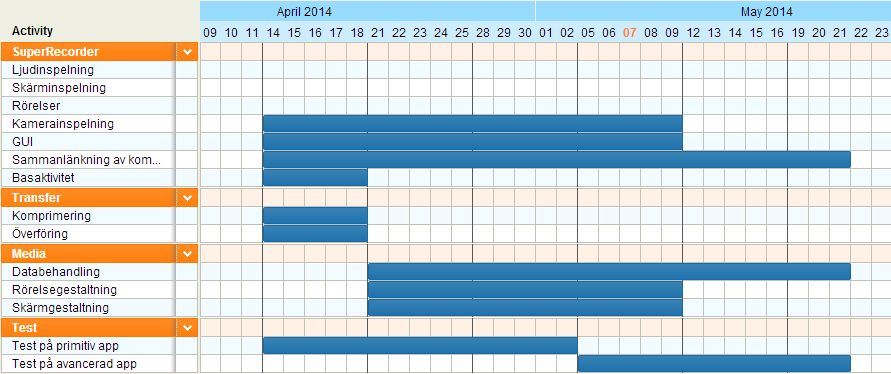
\includegraphics[scale=0.5]{GANTT.png}

\subsection{Individuell veckoplanering}

\begin{tabular}{ | p{100pt} || p{100pt} | p{100pt} | p{100pt} |}
  \hline
  \textbf{Vecka} & 16 & 17 & 18\\ \hline
  \textbf{Daniel Bergström} & Leda programmeringsarbetet och arbeta med Sammanlänkning & Leda programmeringsarbetet och arbeta med Sammanlänkning & Leda programmeringsarbetet och arbeta med Sammanlänkning\\ \hline
  \textbf{Paulina Hensman} & Leda projektet och arbeta med URD-2 & Leda projektet och arbeta med URD-2 & Färdigställa och presentera URD2\\ \hline
  \textbf{Marcus Hertz} & Sammanlänkning & Sammanlänkning & Test, primitiva \\ \hline
  \textbf{Simon Karlsson} & Sammanlänkning av komponeneter & Sammanlänkning av komponeneter & Sammanlänkning av komponeneter\\ \hline
  \textbf{David Masko} & GUI & Färdigställa GUI & Sammanlänkning av komponeneter\\ \hline
  \textbf{Marcus Nordberg} & Rörelsegestaltning & Rörelsegestaltning och URD-2 & Färdigställa och presentera URD2\\ \hline
  \textbf{André Nyström} & Basaktivitet & Databehandling & Databehandling\\ \hline
  \textbf{William Perkola} & Överföring & Databehandling & Databehandling\\ \hline
  \textbf{Axel Riese} & Skärmgestaltning & Skärmgestaltning & Skärmgestaltning\\ \hline
  \textbf{Kerry Zhang} & Hålla kontakt med TBF, arbeta med Komprimering & Hålla kontakt med TBF, arbeta med Databehandling & Hålla kontakt med TBF, arbeta med Databehandling \\ \hline
\end{tabular}

\begin{tabular}{ | p{100pt} || p{110pt} | p{233pt} |}
  \hline
  \textbf{Vecka} & 19 & 20\\ \hline
  \textbf{Daniel Bergström} & Leda programmeringsarbetet, se till att allt blir färdigt & Extratid \\ \hline
  \textbf{Paulina Hensman} & Testning, avancerade appar & Testning, avancerade appar \\ \hline
  \textbf{Marcus Hertz} & Testning, avancerade appar & Extratid \\ \hline
  \textbf{Simon Karlsson} & Färdigställa Sammanlänkning av komponeneter & Extratid\\ \hline
  \textbf{David Masko} & Färdigställa Sammanlänkning av komponeneter & Extratid \\ \hline
  \textbf{Marcus Nordberg} & Färdigställa Sammanlänkning av komponeneter & Extratid \\ \hline
  \textbf{André Nyström} & Färdigställa Databehandling & Extratid \\ \hline
  \textbf{William Perkola} & Färdigställa överföring & Extratid\\ \hline
  \textbf{Axel Riese} & Färdigställa Skärmgestaltning & Slutpresentation \\ \hline
  \textbf{Kerry Zhang} & Hålla kontakt med TBF, förbereda slutpresentation  & Slutpresentation \\ \hline
\end{tabular}



Det finns inte så mycket utrymme för projektet att ta längre tid än planerat. Men tiden som krävs för varje delmoment är uppskattad med god marginal, så det är sannolikt att projektet kommer hamna före schemat. Det finns även utrymme att spendera mer tid per vecka än planerat om det skulle behövas. Projektledaren kommer kontinuerligt att följa upp och justera tidsplaneringen så ingenting blir försenat. Det blir Chief Programmer’s uppgift att sätta upp delmål i programmeringsdelen och följa upp dessa. Projektledaren och Chief Programmer håller nära kontakt.
